\documentclass[11pt]{article}
\usepackage[margin=1in]{geometry}
\usepackage{graphicx}
\usepackage{float}
\usepackage{amsmath,amssymb}
\usepackage{booktabs}
\usepackage[hidelinks]{hyperref}
\usepackage{tikz}
\usetikzlibrary{positioning, arrows.meta}
\tikzset{
  cell/.style={draw, rounded corners, minimum height=7mm, minimum width=11mm, font=\small},
  op/.style={draw, circle, inner sep=1.4pt, font=\footnotesize},
  nz/.style={draw, dashed, rounded corners, minimum height=5mm, minimum width=7mm, font=\scriptsize\itshape},
}

\setlength{\parindent}{0pt}
\setlength{\parskip}{6pt}

\title{\vspace{-1.5cm}Wildfire and Cloud-Forming Particles, Project Midway Report\\
{\large A cumulative summary: models, trust checks, and the causal result}}
\author{Felix Hu, supervised by Prof. Mengxin Yu}
\date{}

\begin{document}
\maketitle
\vspace{-1.1cm}

\section*{The question, in one paragraph}
Marine low clouds cool the planet by reflecting sunlight, and their brightness is governed
largely by the number of cloud-condensation nuclei (CCN, the particles on which cloud
droplets form). How strongly aerosols modify these clouds remains one of the largest
uncertainties in estimates of radiative forcing, chiefly because aerosol and meteorology
are entangled: the weather that carries particles to a site also alters clouds on its own.
Episodic wildfire plumes offer a way in, perturbing an otherwise clean marine environment
over days and hundreds of kilometres, a scale and duration relevant to climate.

Our question is the first link in that chain: does wildfire smoke reaching the Eastern
North Atlantic (ENA) change CCN, and by how much? Wildfires cannot be randomized, so we
turn to generative models: for each 10-day airmass trajectory we learn the \emph{whole
distribution} of CCN it could produce, then compare ``with wildfire'' against ``without''
at the same weather. Because aerosols persist for days, CCN on arrival reflects the history
of the airmass rather than local conditions alone, which is why the trajectory, not the
endpoint, is our unit of analysis. This report covers the models we used, whether we trust
them, and what they say.

This project was motivated by Zhou et al.\footnote{S.~Zhou, D.~Qi, H.~Liu, et al., ``A Lagrangian Time-Series Machine Learning Framework for Predicting Concentrations and Exploring Drivers of Atmospheric Aerosols: Model Development and Application to Cloud Condensation Nuclei in the Marine Boundary Layer,'' AGU Fall Meeting 2024, abstract~1650614, \url{https://agu.confex.com/agu/agu24/meetingapp.cgi/Paper/1650614}; preprint: ESS Open Archive, doi:10.22541/essoar.177038612.23579844.}. That work addresses
prediction; we address causal inference.

\section*{Data and split}
Each sample is a $10$-day back-trajectory timeseries: $241$ hourly steps $\times$ $22$ weather
variables, with target $\log_{10}(\mathrm{CCN})$ at arrival. We use the month-block
(``paper'') split, which mirrors the motivating paper: six alternating months of 2022 are
held out and the remainder used for training.

\begin{center}
\begin{tabular}{lll}
\toprule
& \textbf{Train} & \textbf{Test} \\
\midrule
Trajectories        & $57{,}646$ & $3{,}220$ \\
Wildfire share      & $11.1\%$   & $12.7\%$ \\
Independent episodes & $\sim$2{,}400 & $\sim$135 \\
\bottomrule
\end{tabular}
\end{center}

Two facts carry through the rest of the report: wildfire is a \emph{small minority} of the
data ($\sim$11\%), and adjacent hours are $\sim$99.7\% identical, so tens of thousands of
rows amount to only a few hundred \emph{independent} episodes.

\section*{The models we used}
Everything is an \emph{engression} model: a sampler $\widehat{Y}=g(X,\varepsilon)$ that
takes the weather $X$ plus random noise $\varepsilon$ and returns one possible CCN; draw
it many times and you trace out $P(Y\mid X)$. Training uses the energy-score (CRPS) loss,
which rewards the whole predicted distribution, not just its mean. For the observed
target $y$ and two independent draws $\widehat{Y}=g(X,\varepsilon)$,
$\widehat{Y}'=g(X,\varepsilon')$ from the model,
\[
  \mathcal{L} \;=\; \mathbb{E}\big|\widehat{Y}-y\big|
  \;-\; \tfrac{1}{2}\,\mathbb{E}\big|\widehat{Y}-\widehat{Y}'\big|.
\]
The first term pulls samples toward the truth; the second rewards spread, so the model
cannot collapse to a single point. In practice we minimize its unbiased estimate over $m$
draws $\widehat{y}_1,\dots,\widehat{y}_m$:
\[
  \widehat{\mathcal{L}} \;=\; \frac{1}{m}\sum_{i=1}^{m}\big|\widehat{y}_i-y\big|
  \;-\; \frac{1}{2m(m-1)}\sum_{i\neq j}\big|\widehat{y}_i-\widehat{y}_j\big|.
\]

All three generators we carried into the causal analysis share one skeleton: an
\textbf{LSTM reads the 241-step trajectory}, and a small head turns the result into a
distribution over CCN. What separates them, and makes them stochastic, is
\textbf{where the noise enters the recurrence}:

\begin{itemize}
\item \textbf{Per-timestep.} A fresh, independent $96$-dim noise vector is
\emph{concatenated onto the $22$ weather inputs at every one of the $241$ steps} (so the
LSTM input widens $22\!\to\!118$). Because the noise is redrawn at every step, this variant
resists collapse most effectively of the three.
\item \textbf{Global-latent.} The \emph{same} wiring, except a single $96$-dim code $\varepsilon$ is
drawn \emph{once per trajectory} and concatenated to every step (the same $\varepsilon$ all the way
through), giving one shared ``latent code'' for the whole sequence.
\item \textbf{Recurrent.} The exception: instead of concatenating noise to the inputs,
it uses an \texttt{LSTMCell} and \emph{adds} noise directly to the hidden state after each
step, $h_t \leftarrow h_t + \mathrm{softplus}(s)\,\varepsilon_t$ (with a learned per-unit
scale $s$). Because the state carries forward, the randomness \textbf{accumulates} through
the sequence.
\end{itemize}

\begin{center}
\begin{tabular}{llll}
\toprule
Generator & Noise location & Drawn & Randomness \\
\midrule
Per-timestep  & concat.\ to inputs, each step & fresh each step      & independent per step \\
Global-latent & concat.\ to inputs, each step & once per trajectory  & one shared code \\
Recurrent     & added to hidden state, each step & fresh each step   & accumulates over time \\
\bottomrule
\end{tabular}\\[2pt]
{\footnotesize All three: noise dim $96$, energy-score loss. Swept configs used downstream:
per-timestep $5{\times}128$, global-latent $3{\times}128$, recurrent hidden $192$.}
\end{center}

\begin{figure}[H]
\centering
\textbf{(a) Per-timestep}\; {\footnotesize fresh $\varepsilon_t$ concatenated to the inputs, every step}\\[3pt]
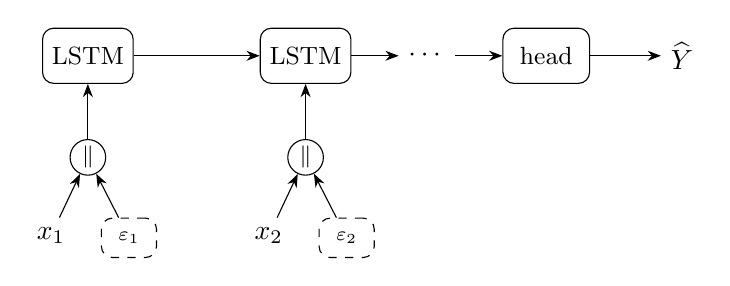
\begin{tikzpicture}[>=Stealth]
  \node[cell] (c1) {LSTM};
  \node[cell, right=16mm of c1] (c2) {LSTM};
  \node[right=6mm of c2] (d) {$\cdots$};
  \node[cell, right=6mm of d] (hd) {head};
  \node[right=9mm of hd] (y) {$\widehat{Y}$};
  \draw[->] (c1)--(c2); \draw[->] (c2)--(d); \draw[->] (d)--(hd); \draw[->] (hd)--(y);
  \node[op, below=7mm of c1] (k1) {$\|$};
  \node[op, below=7mm of c2] (k2) {$\|$};
  \draw[->] (k1)--(c1); \draw[->] (k2)--(c2);
  \node[below left=6mm and 0mm of k1] (x1) {$x_1$};
  \node[nz, below right=6mm and 0mm of k1] (e1) {$\varepsilon_1$};
  \draw[->] (x1)--(k1); \draw[->] (e1)--(k1);
  \node[below left=6mm and 0mm of k2] (x2) {$x_2$};
  \node[nz, below right=6mm and 0mm of k2] (e2) {$\varepsilon_2$};
  \draw[->] (x2)--(k2); \draw[->] (e2)--(k2);
\end{tikzpicture}\\[12pt]
\textbf{(b) Global-latent}\; {\footnotesize one $\varepsilon$ drawn per trajectory, concatenated to every step}\\[3pt]
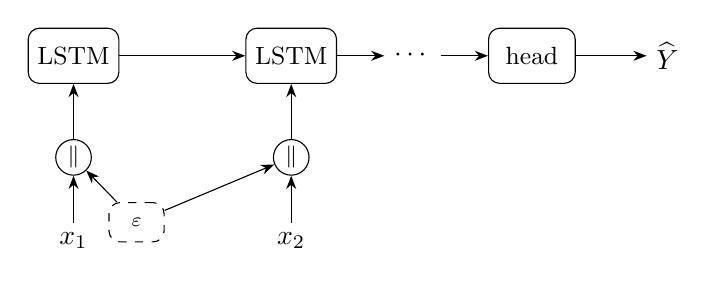
\begin{tikzpicture}[>=Stealth]
  \node[cell] (c1) {LSTM};
  \node[cell, right=16mm of c1] (c2) {LSTM};
  \node[right=6mm of c2] (d) {$\cdots$};
  \node[cell, right=6mm of d] (hd) {head};
  \node[right=9mm of hd] (y) {$\widehat{Y}$};
  \draw[->] (c1)--(c2); \draw[->] (c2)--(d); \draw[->] (d)--(hd); \draw[->] (hd)--(y);
  \node[op, below=7mm of c1] (k1) {$\|$};
  \node[op, below=7mm of c2] (k2) {$\|$};
  \draw[->] (k1)--(c1); \draw[->] (k2)--(c2);
  \node[below=6mm of k1] (x1) {$x_1$};
  \node[below=6mm of k2] (x2) {$x_2$};
  \draw[->] (x1)--(k1); \draw[->] (x2)--(k2);
  \node[nz, below=15mm of c1, xshift=8mm] (z) {$\varepsilon$};
  \draw[->] (z) -- (k1); \draw[->] (z) -- (k2);
\end{tikzpicture}\\[12pt]
\textbf{(c) Recurrent}\; {\footnotesize fresh $\varepsilon_t$ added to the hidden state, accumulating}\\[3pt]
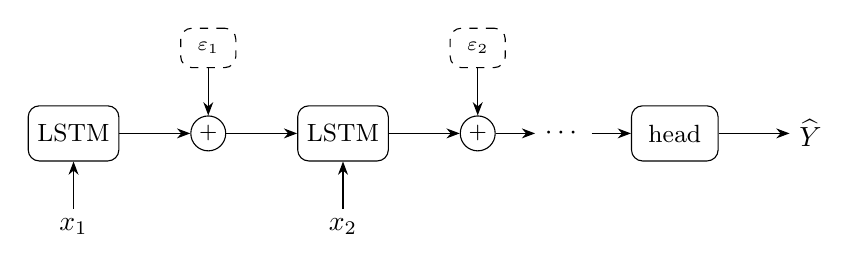
\begin{tikzpicture}[>=Stealth]
  \node[cell] (c1) {LSTM};
  \node[op, right=9mm of c1] (a1) {$+$};
  \node[cell, right=9mm of a1] (c2) {LSTM};
  \node[op, right=9mm of c2] (a2) {$+$};
  \node[right=5mm of a2] (d) {$\cdots$};
  \node[cell, right=5mm of d] (hd) {head};
  \node[right=9mm of hd] (y) {$\widehat{Y}$};
  \draw[->] (c1)--(a1); \draw[->] (a1)--(c2); \draw[->] (c2)--(a2); \draw[->] (a2)--(d); \draw[->] (d)--(hd); \draw[->] (hd)--(y);
  \node[nz, above=6mm of a1] (n1) {$\varepsilon_1$}; \draw[->] (n1)--(a1);
  \node[nz, above=6mm of a2] (n2) {$\varepsilon_2$}; \draw[->] (n2)--(a2);
  \node[below=6mm of c1] (x1) {$x_1$}; \draw[->] (x1)--(c1);
  \node[below=6mm of c2] (x2) {$x_2$}; \draw[->] (x2)--(c2);
\end{tikzpicture}
\caption{Where the noise enters each generator (two steps shown). Inputs $x_t$ rise from
below; the LSTM runs left to right into the head and output $\widehat{Y}$; dashed nodes are
noise. ``$\|$'' concatenates noise to the inputs (a,\,b); ``$+$'' adds it to the hidden
state (c). In (a) the noise is fresh each step; in (b) a single $\varepsilon$ feeds every step; in
(c) it accumulates along the chain.}
\label{fig:arch}
\end{figure}

\section*{Do we trust the models?}
Two checks precede any causal claim.

\textbf{Calibration (PIT).} The \emph{probability integral transform} rests on the fact
behind inverse-transform sampling: if $X$ has CDF $F$, then $F(X)$ is uniform on $[0,1]$.
Passing each observed CCN through its own predicted CDF should therefore yield
\textbf{uniform} values whenever the predicted distribution is correct. In practice the PIT
is the fraction of the model's samples falling below the observed CCN, an empirical $F$. A
well-calibrated model gives a \textbf{flat} histogram, whereas a \textbf{U-shape} indicates
overconfidence, that is, intervals that are too narrow. Across the $48$ sweep
configurations (Figure~\ref{fig:pit}) most histograms are mildly U-shaped and the best are
nearly flat. All histograms and $A^2$ statistics below use the full held-out test set of
$3{,}220$ trajectories, with $400$ predictive draws per trajectory and no subsampling.

\begin{figure}[H]
\centering
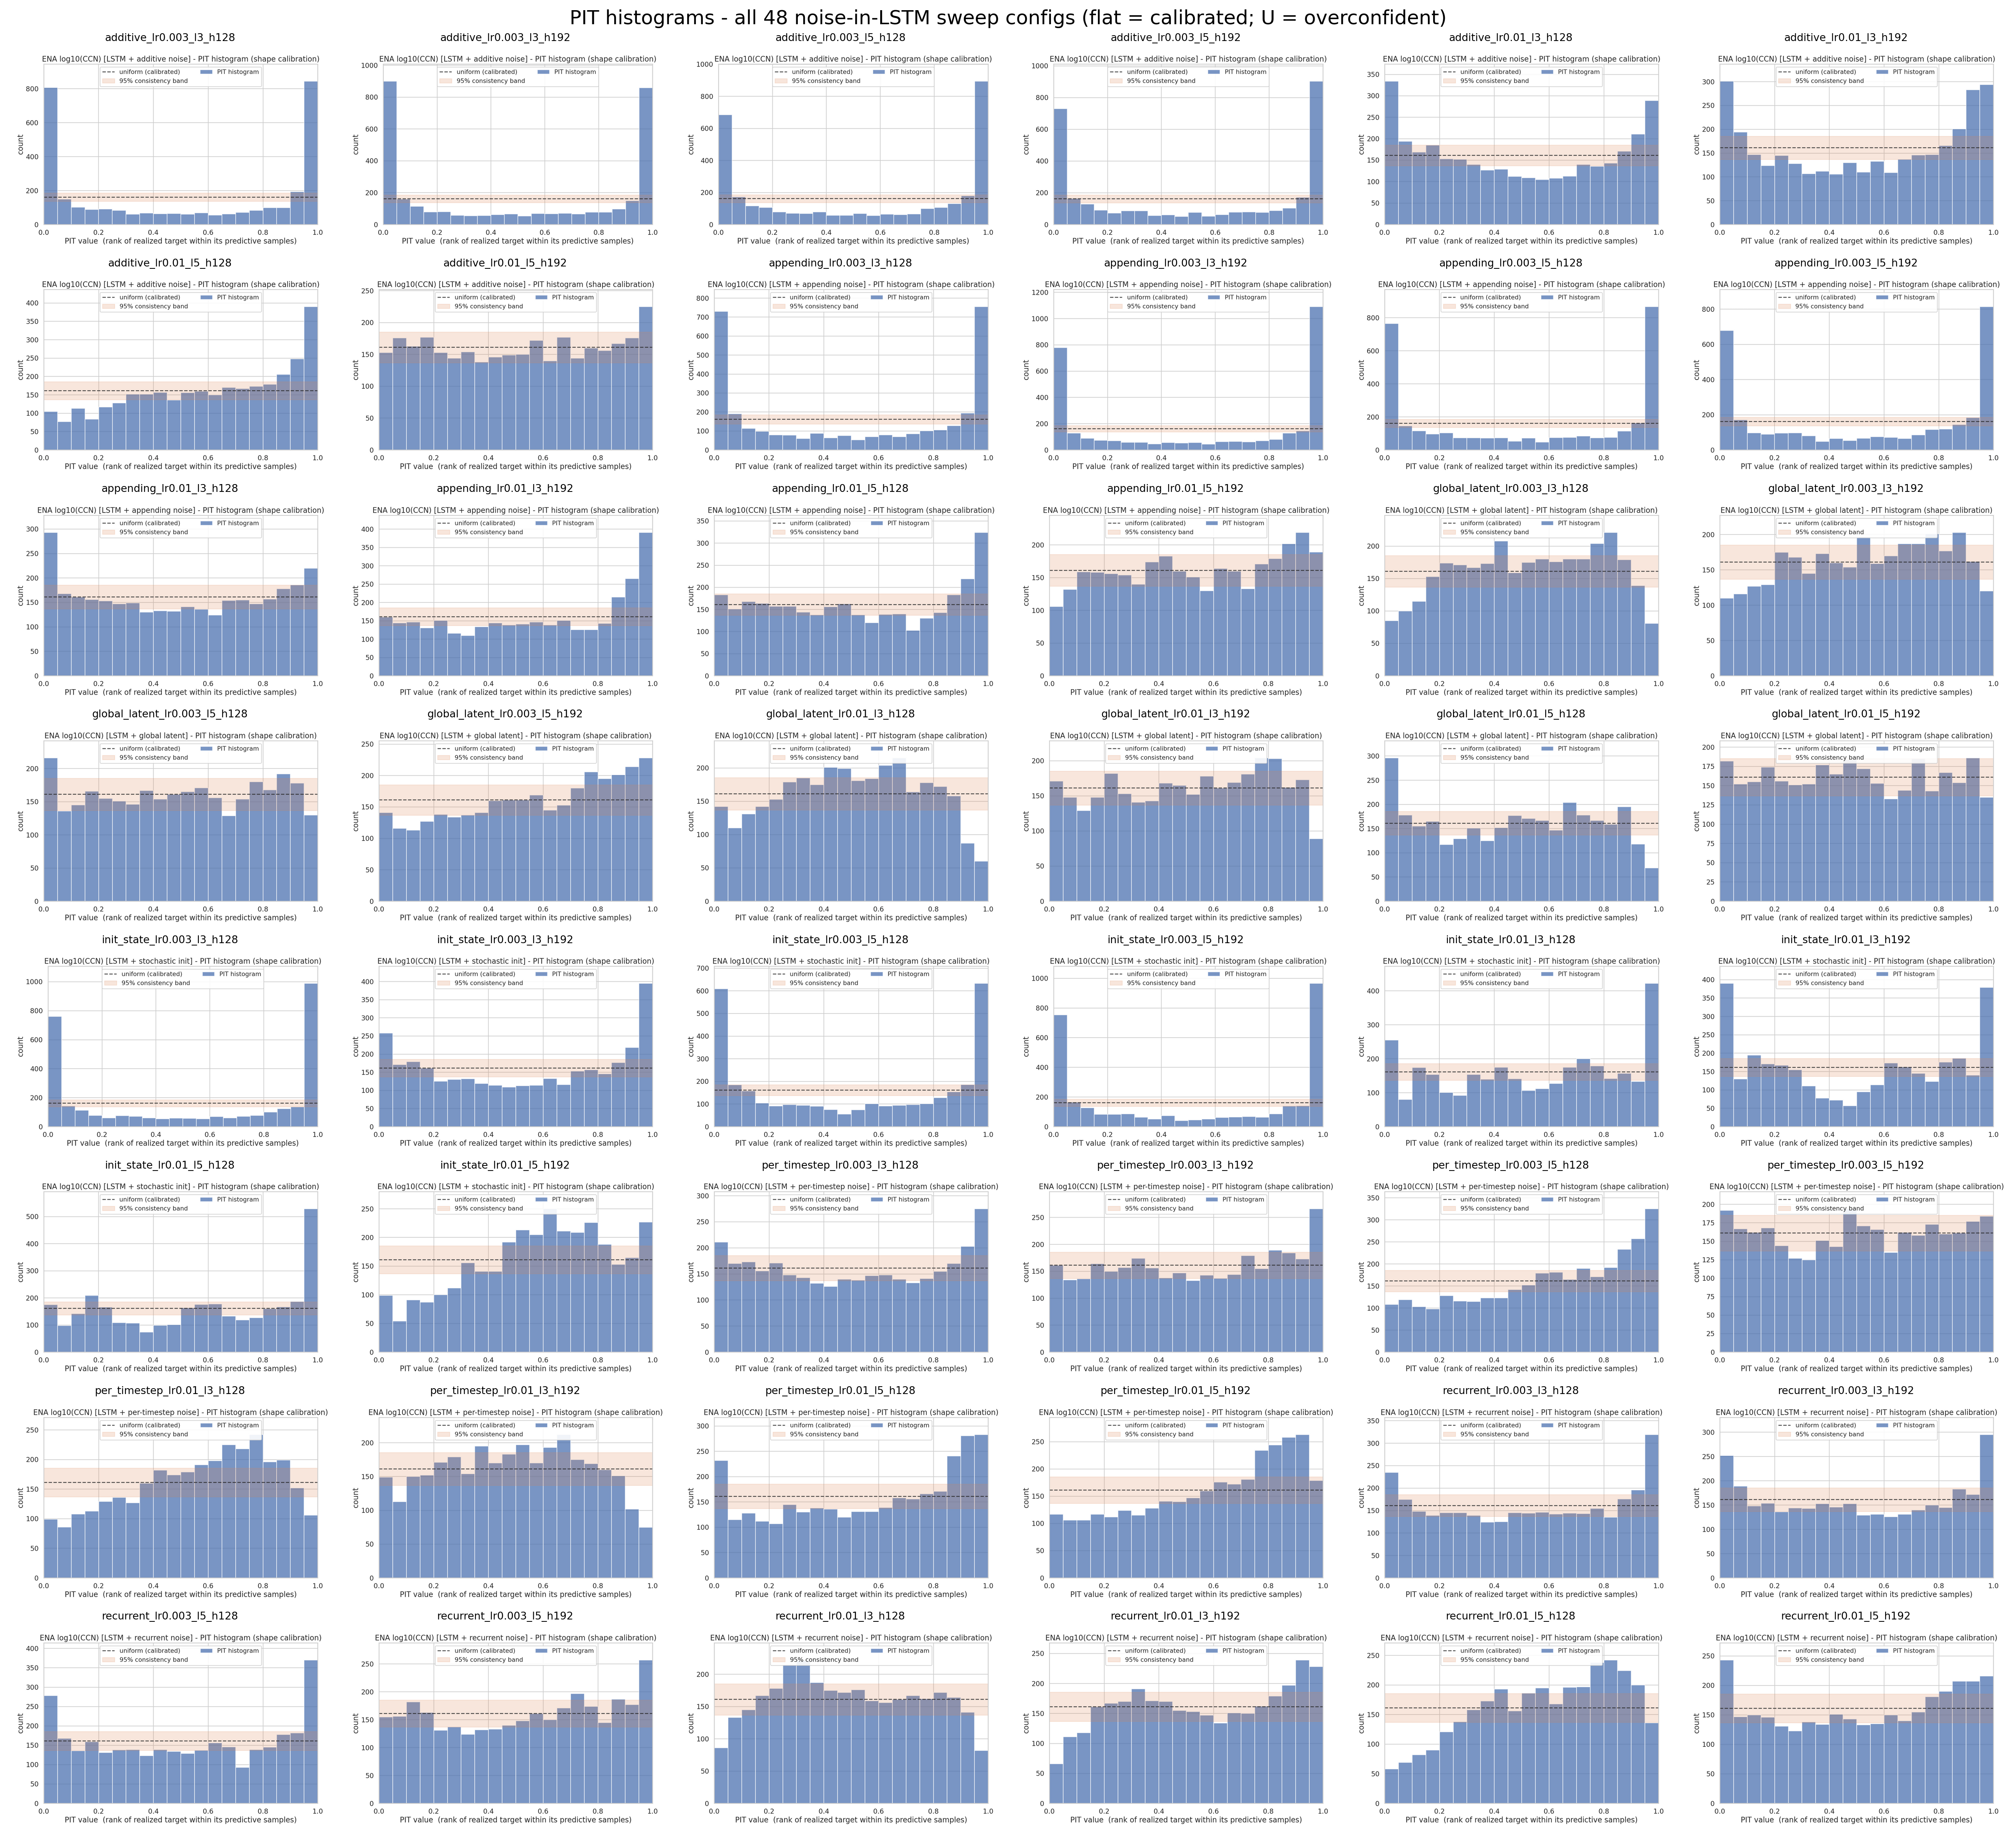
\includegraphics[width=0.95\textwidth]{pit_grid_48.png}
\caption{PIT histograms for all 48 configs. Flat = calibrated; U-shape = overconfident.
Most are mildly U-shaped, the best near flat.}
\label{fig:pit}
\end{figure}

\textbf{Quantifying uniformity.} To move beyond visual inspection of the $48$ histograms,
we summarize each with the Anderson--Darling statistic $A^2$, a scalar measure of a
sample's departure from uniformity. Under correct calibration $A^2$ has expectation near
unity, and it grows as the histogram becomes more U-shaped. As an informal guide,
$A^2\lesssim 2.5$ is indistinguishable from uniform, values in the tens indicate a visible
departure, and values in the hundreds or beyond indicate pronounced overconfidence. The
table below reports, for each noise variant, the best, median, and worst $A^2$ over its
eight swept configurations.

\begin{center}
\begin{tabular}{lccc}
\toprule
Noise variant & Best $A^2$ & Median $A^2$ & Worst $A^2$ \\
\midrule
Global-latent   & \textbf{1.0} & \textbf{23.8} & \textbf{56.4} \\
Per-timestep    & 3.8  & 46.5  & 170.6 \\
Additive        & 6.1  & 601.9 & 1252.6 \\
Recurrent       & 16.3 & 37.6  & 128.4 \\
Appending       & 20.0 & 482.9 & 1583.3 \\
Stochastic-init & 96.0 & 251.2 & 1661.6 \\
\bottomrule
\end{tabular}\\[2pt]
{\footnotesize Anderson--Darling $A^2$ against the uniform distribution, summarized over the
eight configurations (learning rate $\times$ depth $\times$ width) of each variant and
ordered by best $A^2$. Because consecutive hourly trajectories overlap substantially, $A^2$
is best read as a relative ranking rather than an exact test statistic; only the values in
the hundreds and above correspond to unambiguous miscalibration.}
\end{center}

The global-latent generator is the best calibrated of the six: it attains the lowest score
($A^2=1.0$, effectively uniform) and never exceeds $56$ anywhere in the sweep. The
per-timestep and recurrent variants are also consistently well calibrated, which supports
their use as the downstream generators. The remaining three variants can degrade to severe
overconfidence, with $A^2$ reaching the thousands; these failures arise exclusively at the
smaller learning rate ($0.003$), while the same architectures trained at the larger rate
remain well calibrated.

\textbf{Is the test weather in-distribution?} The 2022 test weather differs significantly
from the training weather: a classifier separates the two at AUC $0.79$, and an MMD
permutation test gives $p=0.0008$, driven mostly by carbon monoxide, a smoke tracer.
Different, however, is not the same as unseen. Test trajectories still lie \emph{inside}
the training region (nearest-neighbour distance ratio $1.04$, with only $7.4\%$ beyond the
training 95th percentile; Figure~\ref{fig:shift}), so the overlap the causal comparison
requires does hold.

\begin{figure}[H]
\centering
\begin{minipage}{0.48\textwidth}\centering
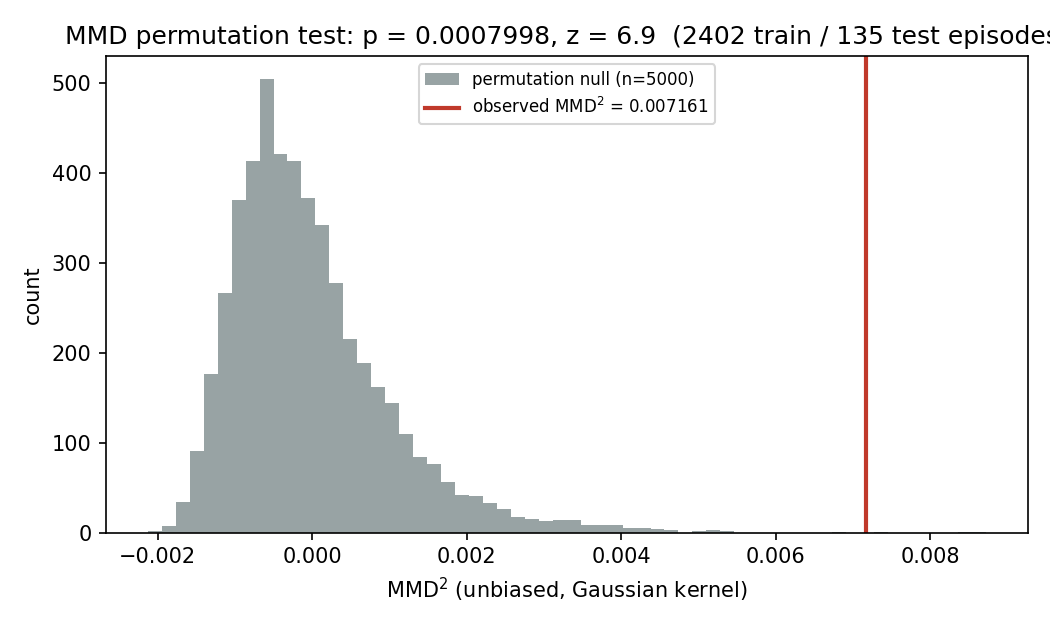
\includegraphics[width=\textwidth]{mmd_null.png}\\[-0.2em]{\small (a) MMD: shift is real}
\end{minipage}\hfill
\begin{minipage}{0.48\textwidth}\centering
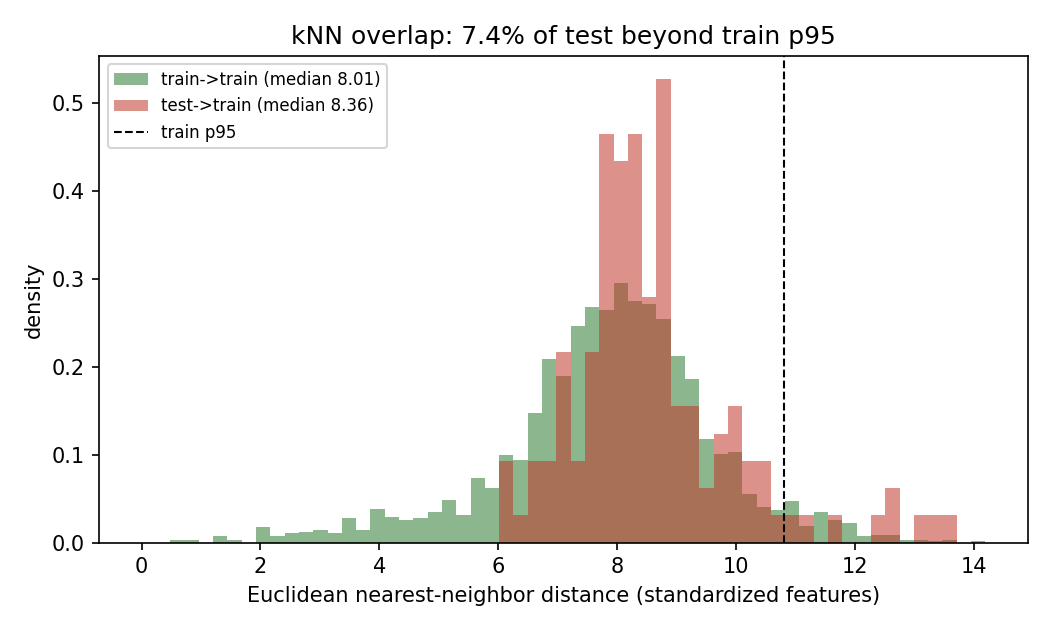
\includegraphics[width=\textwidth]{knn_overlap.png}\\[-0.2em]{\small (b) but test stays in-support}
\end{minipage}
\caption{(a) Observed MMD (red) sits far outside the ``no difference'' null (grey): the
train/test shift is statistically real. (b) Yet test$\to$train distances (red) track
train$\to$train (green): the test weather stays inside the training region.}
\label{fig:shift}
\end{figure}

\section*{What relates to CCN?}
No single variable drives CCN (Figure~\ref{fig:corr}). The strongest correlate is
downwelling solar radiation (\texttt{SWGDN}, $+0.33$), followed by cloud water, low cloud,
and wind speed (all $\approx-0.25$); particles are more abundant on sunny, calm, low-cloud
days. Pearson and Spearman correlations are nearly identical, so the marginal relationships
are close to linear and the nonlinearity lies in how the variables combine. \texttt{CO}
deserves separate mention: although it separates train from test more sharply than any
other variable, it barely correlates with CCN on its own. It marks \emph{when} smoky air
arrives rather than how much CCN is present.

\begin{figure}[H]
\centering
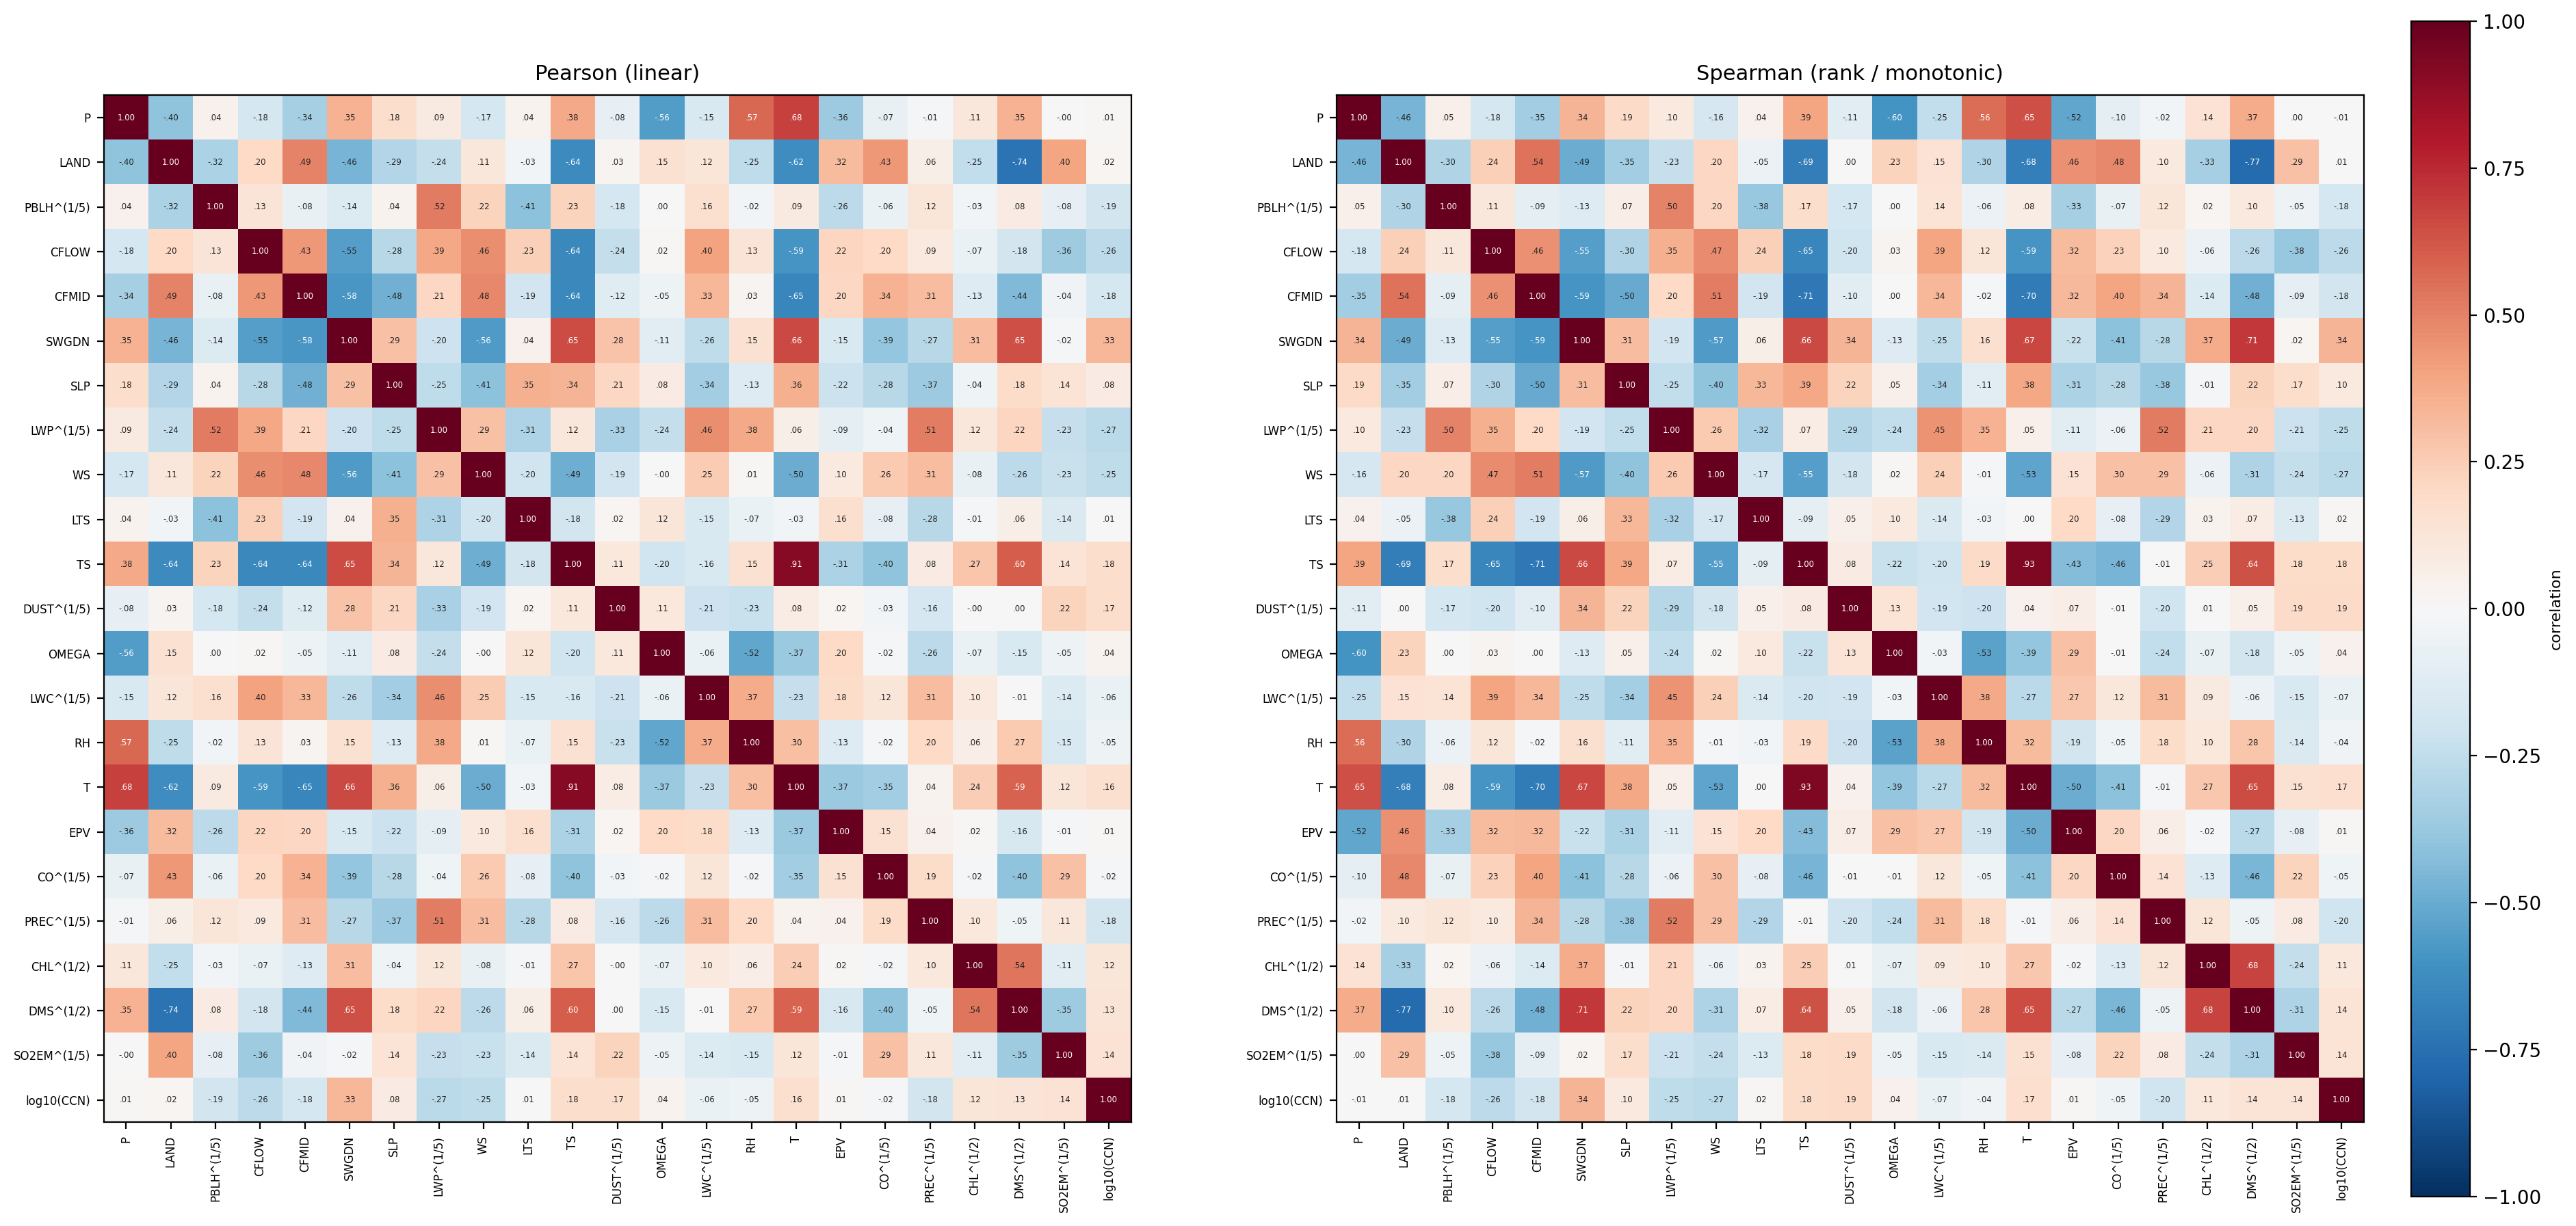
\includegraphics[width=0.92\textwidth]{correlation_heatmap.png}
\caption{Correlation of all 23 variables (per-sample trajectory means, $20{,}000$ samples).
Left = Pearson (linear), right = Spearman (rank). Their near-identity means the marginal
relationships are close to monotone-linear.}
\label{fig:corr}
\end{figure}

\section*{Covariates sensitive to wildfire}
The covariates divide into two groups: those negligibly affected by smoke
(\emph{wildfire-robust}) and those that shift measurably during wildfire periods
(\emph{wildfire-sensitive}). The distinction matters twice over. Sensitive variables are
potential confounders, and their unperturbed values during wildfire periods are never
observed, so any counterfactual conditioning on them must model those values rather than
read them off. We therefore examine all $22$, comparing for each the distribution inside
wildfire periods (\texttt{BB\_criterion1}, the same treatment definition used by the
T-learner; $6{,}786$ trajectories) against outside them, taking the per-trajectory mean as
the sample unit, consistent with Figure~\ref{fig:corr}.

\textbf{Season confounds the naive comparison.} Wildfire periods are strongly seasonal:
$84\%$ of wildfire trajectories arrive between June and September, and January and December
contain none at all. The wildfire-free group is therefore weighted toward winter, so any
covariate with an annual cycle differs between the two groups whether or not smoke affects
it. Comparing the raw distributions largely recovers the seasonal cycle. To break that
confound we repeat every comparison against a \emph{month-matched} subsample of
wildfire-free trajectories, drawn to reproduce the wildfire group's calendar-month
distribution ($17{,}337$ trajectories); season can then no longer explain a difference.

Three measures quantify each difference: the two-sample Anderson--Darling statistic $A^2$
(scale-free and tail-sensitive), the Wasserstein-1 distance, and the energy distance. The
distances carry the covariate's units, so the table reports them standardized by the pooled
standard deviation $\hat\sigma$: $W_1/\hat\sigma$ is the average displacement between the
two distributions measured in standard deviations, and the energy distance is squared
before standardizing so that the ratio is dimensionless. Once standardized the three agree
closely (pairwise Spearman correlations of about $0.99$), so the ordering does not depend
on the choice of statistic. Because the samples are large and temporally autocorrelated,
nearly every test is formally significant; the statistics are best read as a ranking of
shift severity rather than as tests.

\begin{center}
\scriptsize
\setlength{\tabcolsep}{2.6pt}
\begin{tabular}{lrrrrrrrrrrrrrr}
\toprule
& \multicolumn{2}{c}{$A^2$} & & & \multicolumn{5}{c}{Wildfire quantiles (\%)} & \multicolumn{5}{c}{Matched wildfire-free (\%)} \\
\cmidrule(lr){2-3}\cmidrule(lr){6-10}\cmidrule(lr){11-15}
Covariate & raw & matched & $W_1/\hat\sigma$ & $E^2/\hat\sigma$ & 5 & 25 & 50 & 75 & 95 & 5 & 25 & 50 & 75 & 95 \\
\midrule
\texttt{CO}$^{1/5}$ & 331 & 2037 & 0.787 & 0.369 & 0.037 & 0.039 & 0.040 & 0.041 & 0.044 & 0.037 & 0.038 & 0.039 & 0.040 & 0.042 \\
\texttt{LAND} & 59 & 768 & 0.440 & 0.134 & 0 & 0.0041 & 0.137 & 0.290 & 0.485 & 0 & 0 & 0.029 & 0.178 & 0.407 \\
\texttt{PBLH}$^{1/5}$ & 825 & 593 & 0.417 & 0.113 & 3.17 & 3.35 & 3.50 & 3.65 & 3.85 & 3.22 & 3.46 & 3.61 & 3.74 & 3.91 \\
\texttt{LWP}$^{1/5}$ & 387 & 491 & 0.420 & 0.097 & 0.276 & 0.397 & 0.478 & 0.541 & 0.612 & 0.363 & 0.452 & 0.507 & 0.558 & 0.623 \\
\texttt{DMS}$^{1/2}$ & 1038 & 451 & 0.330 & 0.075 & 0.671 & 0.968 & 1.21 & 1.41 & 2.02 & 0.724 & 1.15 & 1.30 & 1.59 & 2.11 \\
\texttt{SLP} (${\times}10^{5}$) & 305 & 350 & 0.303 & 0.066 & 1.010 & 1.014 & 1.018 & 1.021 & 1.026 & 1.010 & 1.015 & 1.019 & 1.023 & 1.028 \\
\texttt{P} & 99 & 253 & 0.230 & 0.042 & 746 & 846 & 905 & 956 & 1002 & 754 & 866 & 927 & 981 & 1009 \\
\texttt{EPV} (${\times}10^{-7}$) & 87 & 247 & 0.192 & 0.033 & $-0.04$ & 2.66 & 4.18 & 5.84 & 9.55 & $-0.60$ & 1.56 & 3.47 & 5.42 & 9.32 \\
\texttt{SO2EM}$^{1/5}$ & 77 & 196 & 0.228 & 0.031 & 0.00053 & 0.001 & 0.0015 & 0.0022 & 0.0036 & 0.00038 & 0.00081 & 0.0013 & 0.002 & 0.0031 \\
\texttt{RH} & 39 & 156 & 0.214 & 0.031 & 0.541 & 0.665 & 0.747 & 0.812 & 0.876 & 0.559 & 0.702 & 0.770 & 0.825 & 0.885 \\
\texttt{CHL}$^{1/2}$ & 1195 & 145 & 0.270 & 0.024 & 0.259 & 0.346 & 0.441 & 0.570 & 0.951 & 0.234 & 0.315 & 0.426 & 0.536 & 0.724 \\
\texttt{CFLOW} & 1081 & 143 & 0.200 & 0.027 & 0.064 & 0.162 & 0.273 & 0.394 & 0.581 & 0.080 & 0.196 & 0.313 & 0.430 & 0.597 \\
\texttt{DUST}$^{1/5}$ & 8 & 130 & 0.176 & 0.020 & 0.0091 & 0.010 & 0.012 & 0.013 & 0.015 & 0.0086 & 0.0099 & 0.011 & 0.013 & 0.015 \\
\texttt{OMEGA} & 0 & 108 & 0.192 & 0.021 & $-0.013$ & 0.0018 & 0.015 & 0.031 & 0.051 & $-0.011$ & $-0.0003$ & 0.012 & 0.025 & 0.047 \\
\texttt{TS} & 2107 & 80 & 0.160 & 0.014 & 279 & 285 & 290 & 294 & 298 & 276 & 284 & 289 & 295 & 299 \\
\texttt{PREC}$^{1/5}$ & 21 & 76 & 0.134 & 0.013 & 0.035 & 0.087 & 0.136 & 0.195 & 0.285 & 0.026 & 0.073 & 0.124 & 0.184 & 0.284 \\
\texttt{CFMID} & 1076 & 67 & 0.118 & 0.008 & 0.011 & 0.046 & 0.086 & 0.141 & 0.232 & 0.0041 & 0.036 & 0.085 & 0.149 & 0.261 \\
\texttt{WS} & 1515 & 67 & 0.140 & 0.013 & 3.68 & 4.61 & 5.31 & 6.13 & 7.33 & 3.67 & 4.70 & 5.49 & 6.35 & 7.70 \\
\texttt{T} & 1757 & 56 & 0.130 & 0.010 & 269 & 279 & 284 & 290 & 296 & 266 & 278 & 285 & 291 & 297 \\
\texttt{SWGDN} & 2199 & 45 & 0.101 & 0.006 & 112 & 185 & 231 & 268 & 309 & 99.1 & 179 & 231 & 277 & 320 \\
\texttt{LWC}$^{1/5}$ & 13 & 33 & 0.073 & 0.004 & 0.0054 & 0.026 & 0.043 & 0.062 & 0.086 & 0.0012 & 0.025 & 0.044 & 0.063 & 0.089 \\
\texttt{LTS} & 89 & 4 & 0.038 & 0.001 & 13.1 & 15.5 & 17.0 & 18.5 & 21.0 & 13.1 & 15.5 & 17.0 & 18.6 & 20.6 \\
\bottomrule
\end{tabular}\\[2pt]
{\footnotesize Per-covariate comparison of wildfire vs wildfire-free trajectories
(per-trajectory means), ordered by the month-matched $A^2$. The ``raw'' column compares
against all $54{,}080$ wildfire-free trajectories; every other column compares against the
month-matched subsample, as do the quantiles shown. The distance columns are standardized:
$W_1/\hat\sigma$ and $E^2/\hat\sigma$ divide the Wasserstein-1 distance and the squared
energy distance by the covariate's pooled standard deviation, so both are dimensionless and
comparable across rows ($A^2$ is scale-free by construction). Quantiles are on each
covariate's stored (power-transformed) scale, with \texttt{SLP} and \texttt{EPV} scaled as
indicated.}
\end{center}

Matching on month reorders the table almost completely, which is the main lesson of this
section. The four covariates that dominate the raw comparison are precisely those with the
strongest annual cycles, and they collapse once season is held fixed: \texttt{SWGDN} falls
from $A^2=2199$ to $45$ (first place to twentieth), \texttt{T} from $1757$ to $56$, and
\texttt{TS} and \texttt{WS} similarly. Their apparent sensitivity to wildfire was largely
the summer climatology of the Azores. The ocean-biology terms \texttt{CHL} and \texttt{DMS}
fall for the same reason.

What rises is more physically suggestive. \texttt{CO}, a long-range tracer of biomass
burning, moves from eleventh to first with $A^2$ increasing sixfold, and \texttt{LAND}, the
fraction of the trajectory spent over land, from seventeenth to second. Together these
describe continental air that has passed over burning regions, which is what a smoke
signature should look like. \texttt{PBLH} and \texttt{LWP}, both plausible responses to
absorbing aerosol aloft, remain high after matching. Note also that \texttt{CO} achieves
the largest matched $A^2$ in the table while its central quantiles stay nearly unchanged:
its shift lives in the upper tail, in the smoke episodes themselves, where a tail-sensitive
statistic sees what quantiles near the median cannot.

Even so, this table cannot by itself identify wildfire-sensitive variables, and the
\texttt{LAND} result shows why. Smoke does not alter the fraction of a trajectory spent
over land; rather, trajectories that cross land are the ones that collect smoke. A
month-matched difference still conflates ``smoke changes this variable'' with ``smoke
arrives in air masses that already differ in this variable.'' Season is only the most
obvious such confounder, not the only one. Separating the two requires exactly the
machinery the next section applies to CCN: a model of what each variable would have been in
the same air mass without the smoke.

\section*{The result: wildfire raises CCN}
We use a \textbf{T-learner}: one model is trained on wildfire trajectories and another on
wildfire-free ones, and \emph{both} are then run on the same weather. The wildfire arm
gives the observed ``with smoke'' CCN, the clean arm gives the counterfactual ``what it
would have been without,'' and the gap between them is the wildfire effect. Both arms use
the stochastic LSTM generators described above, and the entire T-learner is run once per
architecture: per-timestep ($5\times128$), global-latent ($3\times128$), and recurrent
(hidden $192$). Each row below, and each effect plot, is therefore one complete two-arm
T-learner.

Our primary estimate is the \textbf{ATE (average treatment effect)}, which averages over
\emph{all} test weather and so captures the typical effect of wildfire across conditions.
\textbf{Wildfire raises CCN by roughly 20--30\%} ($\approx +30$ to $+40$ particles
cm$^{-3}$), with the whole distribution shifting upward and developing a heavier upper tail
(Figure~\ref{fig:money}). All three generators agree:

\begin{center}
\begin{tabular}{lcc}
\toprule
Generator & \textbf{ATE} (all weather) & ATT (wildfire weather) \\
\midrule
Per-timestep  & $+20\%$ & $+10\%$ \\
Recurrent     & $+31\%$ & $+16\%$ \\
Global-latent & $+31\%$ & $+24\%$ \\
\bottomrule
\end{tabular}
\end{center}

\begin{figure}[H]
\centering
\begin{minipage}{0.32\textwidth}\centering
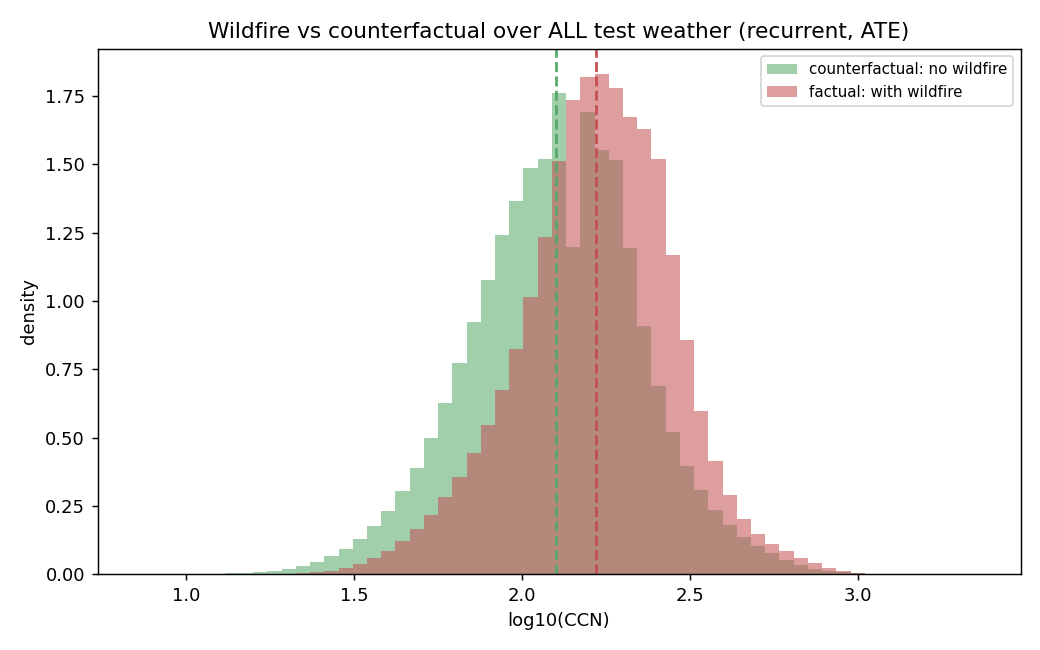
\includegraphics[width=\linewidth]{money_recurrent_ate.png}\\{\small recurrent: $+31\%$}
\end{minipage}\hfill
\begin{minipage}{0.32\textwidth}\centering
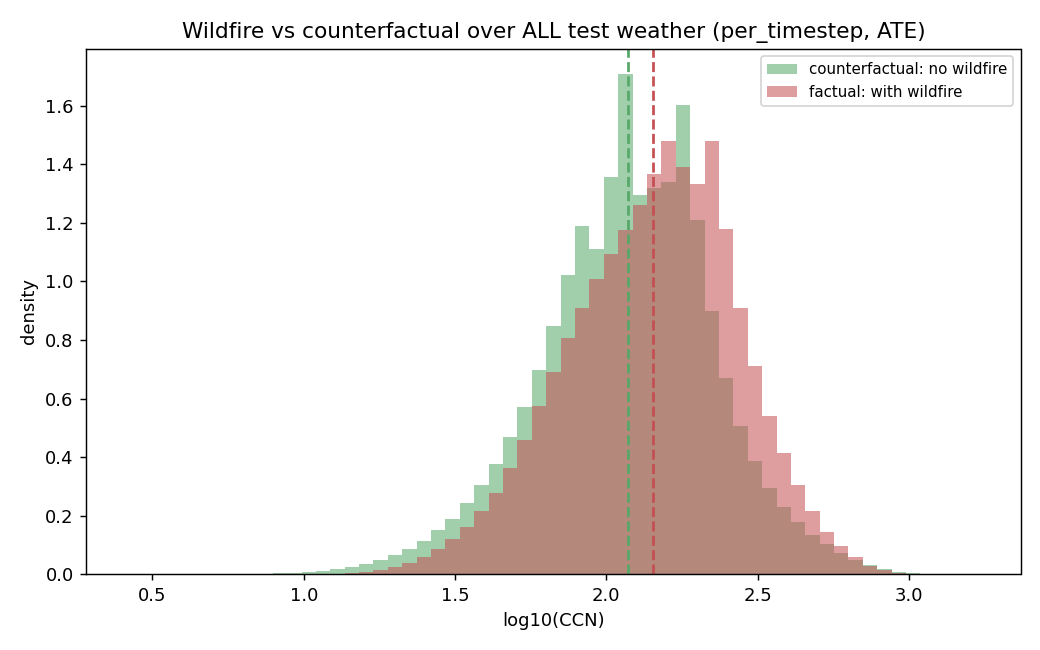
\includegraphics[width=\linewidth]{money_per_timestep_ate.png}\\{\small per-timestep: $+20\%$}
\end{minipage}\hfill
\begin{minipage}{0.32\textwidth}\centering
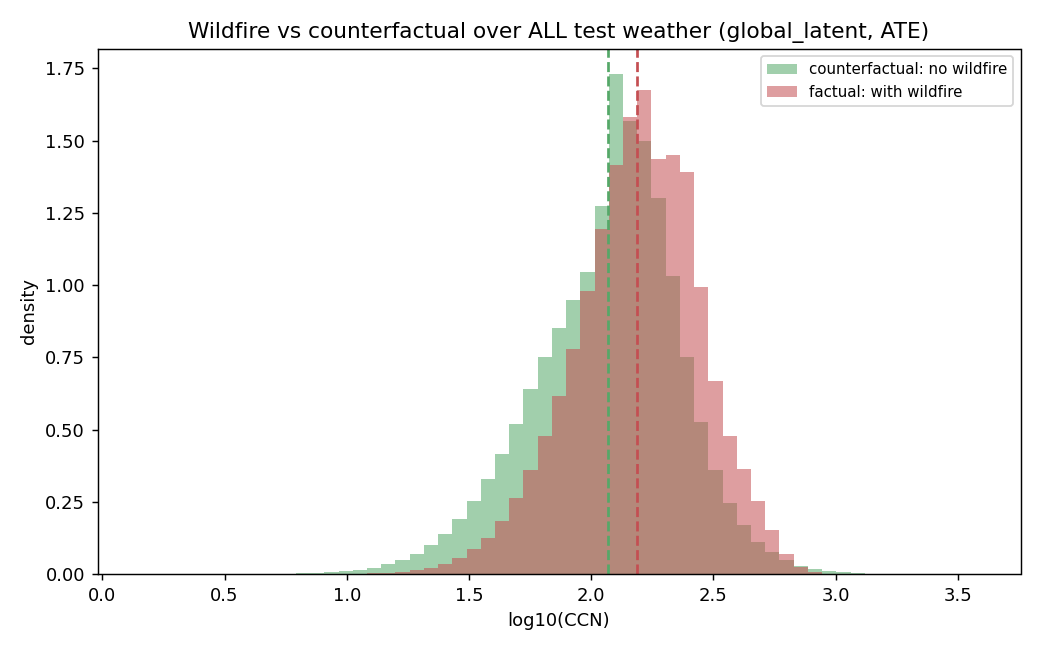
\includegraphics[width=\linewidth]{money_global_latent_ate.png}\\{\small global-latent: $+31\%$}
\end{minipage}
\caption{ATE view: CCN with wildfire (red) vs.\ the counterfactual without (green),
both evaluated over \emph{all} held-out test weather. Every generator shifts the
distribution up (dashed = means) with a fatter high tail. Horizontal axis is a log scale.}
\label{fig:money}
\end{figure}

\textbf{ATE and ATT.} The ATT (right column) restricts the effect to weather that actually
occurred \emph{during} wildfire periods, and is smaller ($+10$ to $+24\%$). The ATE is
larger because it also asks what wildfire would do on \emph{clean}-weather days, which
requires the wildfire arm to predict on conditions it rarely saw; part of the gap between
the two therefore reflects extrapolation. The ATE is best read as the broad average effect
and the ATT as the conservative, in-support estimate.

\section*{Caveats and bottom line}
The estimate rests on ignorability: the $22$ weather variables must capture everything that
differs between wildfire and clean air apart from the smoke itself. There are no formal
error bars yet, and the number of independent wildfire episodes is far smaller than the
number of observations, so $+20\%$ to $+31\%$ should be read as a range rather than as
exact figures. Because the ATE averages over all conditions, it also depends in part on the
data-poor wildfire arm extrapolating onto clean weather.

\textbf{Bottom line.} Across three stochastic generators, wildfire smoke raises
cloud-forming particles at ENA by roughly \textbf{20--30\%} on average (ATE), or a more
conservative \textbf{10--24\%} when restricted to wildfire conditions (ATT). The models are
reasonably calibrated and the test weather remains in support, so the direction and
approximate magnitude of the effect are well founded. CCN is only the first link in the
chain from smoke to cloud brightness; carrying the same counterfactual machinery through to
cloud properties themselves is the natural next step.

\end{document}
